\documentclass[twocolumn,amsmath,amssymb,floatfix]{revtex4}

\usepackage{graphicx}% Include figure files
\usepackage{dcolumn}% Align table columns on decimal point
\usepackage{bm}% bold math
\usepackage{amssymb}
\usepackage{amsmath}
\usepackage{amsfonts}
\usepackage{epsf}
\usepackage{color} % allows color in fonts
\usepackage{verbatim}
\usepackage{listings}
\usepackage{xcolor}
\usepackage{titlesec}
\usepackage{float}
\usepackage[most]{tcolorbox}
\usepackage[brazilian]{babel}
\usepackage[utf8]{inputenc}
\usepackage[T1]{fontenc}

\newcommand{\PAR}[1]{\left({[#1]}\right)}


\lstdefinestyle{customc}{
  belowcaptionskip=1\baselineskip,
  breaklines=true,
  frame=none,
  xleftmargin=\parindent,
  language=C,
  showstringspaces=false,
  basicstyle=\footnotesize\ttfamily,
  keywordstyle=\bfseries\color{green!40!black},
  commentstyle=\itshape\color{purple!40!black},
  identifierstyle=\color{blue},
  stringstyle=\color{orange},
}

\lstdefinestyle{customasm}{
  belowcaptionskip=1\baselineskip,
  frame=trBL,
  xleftmargin=\parindent,
  language=[x86masm]Assembler,
  basicstyle=\footnotesize\ttfamily,
  commentstyle=\itshape\color{purple!40!black},
}

\lstset{escapechar=@,style=customc}

\titlespacing\section{0pt}{12pt plus 4pt minus 2pt}{8pt plus 2pt minus 2pt}
\titlespacing\subsection{0pt}{12pt plus 4pt minus 2pt}{8pt plus 2pt minus 2pt}
\titlespacing\subsubsection{0pt}{12pt plus 4pt minus 2pt}{0pt plus 2pt minus 2pt}

\definecolor{bg}{RGB}{255,249,227}

\begin{document}

%%%%%%%%%%%%%%%%%%%%%%
% T I T U L O
%%%%%%%%%%%%%%%%%%%%%%

\title{Implementação de um Classificador de Digitos MNIST}

\author{Lucas Penna Saraiva e Stefan Radzciczyj Raposo \\\small lucas.saraiva@usp.br stefanraposo@usp.br}
\affiliation{
Escola Politécnica da Universidade de São Paulo\\
Instituto de Matemática e Estatística\\
Departamento de Matemática Aplicada
}

\begin{abstract}
\baselineskip 11pt
O aprendizado de máquinas, \textit{machine learning}, é um campo de estudos da ciência da computação, aplicando teorias de inteligência artificial. Nesse trabalho, o objetivo foi implementar uma possível técnica de aprendizado de máquina, utilizando fatoração de matrizes, aplicando-se o método na base de dados MNIST, com a finalidade de classificar imagens de dígitos. 
\end{abstract}

\maketitle

%%%%%%%%%%%%%%%%%%%%%%
%%%%%%%%%%%%%%%%%%%%%%
\section{Introdução e Conceitos}
%%%%%%%%%%%%%%%%%%%%%%
%%%%%%%%%%%%%%%%%%%%%%
Grande parte das soluções de projetos de aprendizado de máquina utilizam fatoração de matrizes de dados. Dessa forma, para classificar os digitos MNIST (figura 1), far-se-á necessário recorrer a uma técnica de fatoração. Nesse caso, busca-se fatorar uma dada matriz A pelo produto de duas matrizes (W e H), com certas características que possibilitem a classificação dos dados. Trata-se de uma fatoração não negativa, adequada para o tratamento de dados de imagens. Ao longo do relatório, será discutido com mais detalhes os passos necessários e as técnicas envolvidas para se chegar na fatoração, bem como seu uso na classificação de digitos.

\begin{figure}[h!]
  \centering
  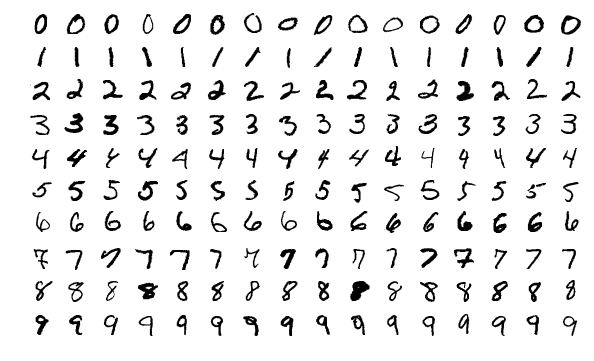
\includegraphics[width=7cm]{MnistExamples.png}
  \caption{Base de dados MNIST}
\end{figure}

%%%%%%%%%%%%%%%%%%%%%%
%%%%%%%%%%%%%%%%%%%%%%
\section{Implementação e testes}
%%%%%%%%%%%%%%%%%%%%%%
%%%%%%%%%%%%%%%%%%%%%%

O desenvolvimento do Classificador MNIST foi feito em \textit{C++}, devido ao fato de ser uma linguagem compilada. Esse fato implica em um ganho de produtividade muito maior para programas que executam um grande volume de operações matemáticas, visto que o ato da compilação gera um arquivo binário. Esse arquivo binário executável encontra muito menos camadas impediditivas para se comunicar com a máquina e cumprir as instruções. As principais bibliotecas de \textit{machine learning} utilizadas atualmente estão implementadas em \textit{Python}, tais como \textit{Scikit Learn} e \textit{Tensorflow}. No entanto, essa implementação se dá apenas no âmbito das funções de alto nível para o usuário final, visto que as tarefas computacionalmente custosas estão implementadas em \textit{C++}. Ou seja, as bibliotecas de alto nível de \textit{Python} possuem otimizações escritas em \textit{C++} de forma a ganhar maior produtividade durante a execução dos algoritmos de aprendizado de máquina.

O projeto do classificador foi estruturado em três arquivos: \textit{"main.cpp"}, \textit{"linearalgebra.h"} e \textit{"interface.h"}. O primeiro arquivo é um arquivo do tipo \textit{".cpp"}, em que se executa as tarefas principais do projeto. Os dois últimos arquivos são arquivos do tipo \textit{".h"} (\textit{header}), onde foram implementadas as funções utilizadas ao longo do projeto. 

No arquivo \textit{"linearalgebra.h"} foram implementadas as principais funções do projeto, como a Rotação de \textit{Givens}, a solução de sistemas simultâneos, a Fatoração QR, a fatoração WH e afins.

As implementações das funções utilizadas na classificação de digitos foram feitas no arquivo \textit{"digitclassifier.h"} e, por fim, no arquivo \textit{"interface.h"} foram implementadas as funções de leitura de arquivos e impressão de matrizes e vetores no terminal.

%%%%%%%%%%%%%%%%%%%%%%
\subsection{Arquivos do projeto}
%%%%%%%%%%%%%%%%%%%%%%

Para o desenvolvimento do projeto, fez-se uso do sistema operacional Linux Ubuntu 16.04 e \textit{workspace} CMake 2.8. As instruções para configuração do ambiente CMake (comandos bash necessários) estão escritos com maior nível de detalhe no arquito README.txt, disponibilizado junto ao projeto. Note que para o \textit{workspace} construíndo no ambiente CMake para a compilação do EP funcionar normalmente depende do sistema operacional. Dessa forma, é fundamental rodar o programa num SO Linux dotado de ambiente CMake. 

Abaixo segue um breve resumo do conte\'udo dos c\'odigos fonte e interfaces.
\\\indent \textbf{main.cpp:} apenas implementa a função main(). Veja o c\'odigo na íntegra no Ap\^endice C.
\\\indent \textbf{interface.h:} implementa as funções de interface. Seu cabeçalho é apresentado a seguir:
\begin{lstlisting}
void printMatrix(float M[MAX_MATRIX][MAX_MATRIX], int m, int n);

void readingFile(std::string filepath, float A[MAX_MATRIX][MAX_MATRIX], int n, int m);

void readingLabel(std::string filepath, int A[MAX_MATRIX], int n);

\end{lstlisting}
\indent \textbf{linearalgebra.h:} implementação dos métodos de álgebra linear numérica. Principais funções:

\begin{lstlisting}

void rotGivens_Matrix(float W[MAX_MATRIX][MAX_MATRIX], int num_Rows, int num_Columns, int i, int j, float c, float s);

void factorizationQR(float A[MAX_MATRIX][MAX_MATRIX], float B[MAX_MATRIX][1], float Result[MAX_MATRIX][1], int num_Rows, int num_Columns);

void overdetermined_systemQR(float W[MAX_MATRIX][MAX_MATRIX], float A[MAX_MATRIX][MAX_MATRIX],
float H[MAX_MATRIX][MAX_MATRIX], int n, int m, int p);

void factorizationWH(float A[MAX_MATRIX][MAX_MATRIX], float W[MAX_MATRIX][MAX_MATRIX], float H[MAX_MATRIX][MAX_MATRIX],
	int m, int n, int p)

\end{lstlisting}

\indent \textbf{digitclassifier.h:} implementação dos métodos relativos à classificação de digitos. Trata-se da biblioteca que contém funções de alto níveis utilizadas para classificar as imagens. Principais funções:

\begin{lstlisting}

void digitClassifier(float A[MAX_MATRIX][MAX_MATRIX], float W[MAX_MATRIX][MAX_MATRIX], float H[MAX_MATRIX][MAX_MATRIX],
	float error[MAX_MATRIX], int digit_predict[MAX_MATRIX],
	int digito, int m, int n, int p);
	
float getAccuracy(int digit_predict[MAX_MATRIX], int digit_correct[MAX_MATRIX], int n_test);

int getNumberOfCorrectPredictions(int digit_predict[MAX_MATRIX], int digit_correct[MAX_MATRIX], int n_test, int digit);

\end{lstlisting}

\subsection{Algoritmos}

Nessa seção, busca-se elucidar com maior detalhe os algoritmos que compõe a solução do projeto, bem como ilustrar com os trechos mais relevantes do código.

\subsection{Rotação de \textit{Givens}}

As Rotações de \textit{Givens} são transformações lineares ortogonais de $R^n$ em $R^n$. A transformação corresponde a uma rotação no plano das coordenadas $i$ e $j$, deixando as outras invanriantes. Aplicando-se a rotação de \textit{Givens} $Q(i, j, \theta)$ a uma matriz $W_{n \times m}$, apenas as linhas $i$ e $j$ são modificadas. As demais linhas não se alteram devido à Rotação de \textit{Givens}.

\begin{figure}[h!]
  \centering
  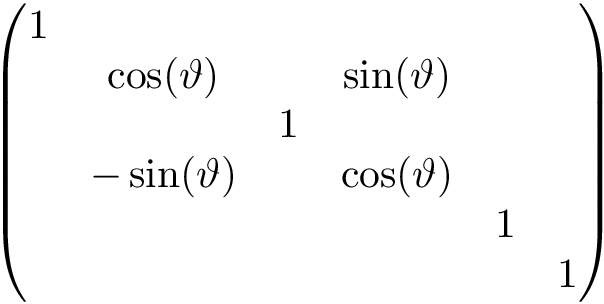
\includegraphics[width=5cm]{GivensMatrix.png}
  \caption{Matriz de \textit{Givens}.}
\end{figure}

Na figura 1 é possível observar a Matrix de Givens, a qual é utilizada para se realizar a transformação. Uma possível implementação seria executar o algoritmo de multiplicação de matrizes entre a matriz $W_{n \times m}$ e Q (figura 1). No entanto, a matriz Q é muito esparsa e seria desperdício de memória. Dessa forma, abaixo uma sugestão para resolver o problema da Rotação de \textit{Givens} implementado em C++:

\begin{lstlisting}
void rotGivens_Matrix(float W[MAX_MATRIX][MAX_MATRIX], int num_Rows, int num_Columns, int i, int j, float c, float s){

	float aux;

	for(int n = 0; n < num_Columns; n++){

		aux = c*W[i][n] - s*W[j][n];
		W[j][n] = s*W[i][n] + c*W[j][n];
		W[i][n] = aux;
	}
}
\end{lstlisting}

\subsection{Fatoração QR}

O objetivo da fatoração QR é transformar uma matriz $W_{n \times m}$ em uma matriz $R_{n \times m}$ com $R_{ij} = 0$, se $i > j$. Dessa forma, ao se aplicar sucessivamente as Rotações de \textit{Givens}, obtemos uma matriz triangular superior. O sistema estará, portanto, escalonado. Trata-se de um algoritmo eficiente para resolver sistemas lineares, porque possui uma complexidade menor do que algoritmos tradicionais como Eliminações de \textit{Gauss}, por exemplo. 

Para que se possa zerar elementos de $W$, é necessário calcular o valor correto de $\theta$ para as linhas $i$ e $j$ para as quais se quer aplicar $Q(i, j, \theta)$. Uma forma de calcular $c = cos(\theta)$ e $s = sin(\theta)$, sugerida no enunciado do problema, implementada, é a seguinte: 

\begin{lstlisting}
void calculateCS(float *c, float *s, float A[MAX_MATRIX][MAX_MATRIX], int i, int j, int k)
{
	float t;
	float c_linha, s_linha;

	if (fabs(A[i][k]) > fabs(A[j][k])){

		t = -(A[j][k]/A[i][k]);

		*c = 1/(sqrt(1+t*t));

		c_linha = *c;

		*s = c_linha * t;
	}
	else{

		t = -(A[i][k])/(A[j][k]);

		*s = 1/(sqrt(1+t*t));

		s_linha = *s;

		*c = s_linha * t;
	}
}
\end{lstlisting}

Em posse da função responsável pelo cálculo dos valores corretos de $c$ e $s$, pode-se partir para a aplicação da função para resolver o problema das sucessivas rotações de givens, com a finalidade de escalonar o sistema. Dessa forma, implementou-se o seguinte loop na função \textit{factorizationQR()}:

\begin{lstlisting}
//for each column
for(int k = 0; k < num_Columns; k++){

	//for each row
	for(int j = num_Rows-1; j > k; j--){

		i = j - 1;

		if(fabs(A[j][k]) > EPSLON){

			calculateCS(&c, &s, A, i, j, k);// CALCULAR C e S para zerar o elemento i,n
			rotGivens_Matrix(A, num_Rows, num_Columns, i, j, c, s);
			rotGivens_Vector(B, i, j, c, s);
		}
	}
}
\end{lstlisting}

Ou seja, percorre-se a matrix de baixo para cima, da esquerda para a direita, zerando todos os elementos de forma a torná-la uma matriz triangular superior, por meio da aplicação de $G \times Wx = G \times B$.
Por fim, a função retorna o vetor $x$ de raízes do sistema linear:

\begin{lstlisting}
	for(int row = num_Rows-1; row >= 0; row--){

		float soma = 0.0;

		for(column = 0; column < num_Columns; column++){

			if(column != row){

				soma = soma + A[row][column] * Result[column][0];

			}
		}

		Result[row][0] = (B[row][0]-soma)/(A[row][row]);

	}
\end{lstlisting}

Nesse caso, o vetor Result armazena as raízes do sistema linear formado por $Wx=B$.

\subsection{Sistemas Simultâneos}

Essa função é uma generalização da função \textit{factorizationQR()} explicada acima. Essa função é responsável por calcular as raízes de sistemas simultâneos $W \times H = A$ , em que $H$ é a matriz que armazena os vetores raízes. A matriz $A$ armazena os múltiplos vetores $B$. Note que os múltiplos sistemas preservam uma mesma característica: possuem a mesma matriz $W$.

Dessa forma, a única alteração em relação a função \textit{factorizationQR()} passa a ser a generalização no último loop, responsável pelo cálculo das raízes do sistema. Nesse caso, é necessário determinar os elementos da matriz $H$. Desse modo, o loop generalizado implementado fica: 

\begin{lstlisting}
for(int k = p-1; k>=0; k--){

	for(int j=0; j<m; j++){

		soma = 0.0;

		for(int i=k+1; i<p; i++){

			soma = soma + W[k][i]*H[i][j];

			}

		H[k][j] = (A[k][j] - soma)/W[k][k];

		}
  	}
}
\end{lstlisting}

\subsection{Fatoração WH}

O problema pode ser compreendido da seguinte maneira: suponha uma matriz $A_{n \times m}$, cujas entradas são positivas ($A$ é uma matriz não negativa). Dado um certo número $p$, deseja-se fatorar $A$ como produto de duas matrizes: $W_{n \times p}$ e $H_{p \times m}$, ambas também positivas. Busca-se tal solução minimizando eventuais erros quadráticos, pois nem sempre há essa fatoração exata para toda matriz dada.

Para solucionar esse problema, foi sugerido no enunciado o método de pontos de mínimos quadrados alternados. Esse método é executado através do seguinte trecho de código, implementado na função \textit{factorizationQR()}:

\begin{lstlisting}

/*Iniciando W randomicamente*/
for(int i = 0; i < n; i++){

	for(int j = 0; j < p; j++){

		W[i][j] = rand();
			}
}
		
/*Armazenando uma copia de A*/
for(int i = 0; i < n; i++){

	for(int j = 0; j < m; j++){

	A_copy[i][j] = A[i][j];
	
	}
}

/* A(n,m)  W(n,p)   H(p,m) */

while(count < ITMAX && error_rate > EPSLON){

	normalizeMatrix(W, n, p);

	for(int i = 0; i < n; i++){

		for(int j = 0; j < m; j++){

			A[i][j] = A_copy[i][j];
			
		}
	}

	overdetermined_systemQR(W, A, H, n, m, p);

	redefine(H, p, m);
		
	transposeMatrix(A_copy, A_transpose, n, m);

    transposeMatrix(H, H_transpose, p, m);

	overdetermined_systemQR(H_transpose, A_transpose, W_transpose, m, n, p); 

	transposeMatrix(W_transpose, W, p, n);

	redefine(W, n, p);

	count = count + 1;
	
	error_rate = erroQuad(A_copy, W, H, n, p, m);
		}
\end{lstlisting}

Ou seja, implementou-se acima em \textit{C++} o seguinte algoritmo de fatorização:

- Inicialize randomicamente $W$;

- Armazene uma cópia de $A$

- Repita até que o erro se estabilize ou número de iterações alcance 100:

\begin{flushright}	

- Normalize $W$;

- Resolva $W \times H = A$; (sistemas simultâneos) 
	
- Redefina $H$; ($H_{i \times j} = max{0, H_{i \times j}}$)

- Calcule transposta de $A$; ($A^t$)

- Resolva $H^t \times W^t = A^t$;

- Calcule transposta de $W^t$;

- Redefina $W$; (da mesma forma que H);

\end{flushright}

\subsection{Treinamento e Classificação dos Digitos}

A etapa de treino foi realizada da seguinte maneira: calculou-se a matriz $W_{d}$ para cada dígito $d = 0, 1, 2, ..., 9$. Ou seja, gera-se 9 matrizes $W$ relativadas a cada dígito treinado. 

A Matriz W é obtida da fatoração WH das matrizes $A$. Nessa matriz $A$ é armazenado o conteúdo do arquivo contendo as imagens de treino para cada dígito. Então, para cada dígito $d$, chama-se a função \textit{factorizationWH()}, da qual se aproveita $W_{d}$ e descarta-se a matriz $H$. Pode-se observar um trecho da implementação a seguir:

\begin{lstlisting}
printf("\n[INFO_MAIN] Treinando o digito 0: \n");

readingFile("/home/lucas/Numerical_Methods/dataset/train_dig0.txt", A, n, m);

factorizationWH(A, W0, H, m, n, p);

\end{lstlisting}

Após obter as matrizes $W_{d}$ na etapa de treino, parte-se para a etapa de testes. Nessa etapa, o objetivo foi classificar os digitos a partir de um arquivo de imagem fornecido. Conhece-se a priori as \textit{labels} das respectivas imagens, tratando-se assim, de um caso de \textit{supervisioned learning}. Assim, após a classificação, conseguimos observar a quantidade de classificações feitas utilizando o arquivo de \textit{labels}.

A classificação é feita da seguinte maneira: para cada coluna $c_{j}$ de $A - W_{d} \times H$ a sua norma euclidiana. Assim, estabelecemos uma métrica para o erro, e baseado no erro, conseguimos efetuar comparações e classificar o digito. Dessa forma, para cada $d$ avaliado, o algoritmo verifica o erro calculado para os digitos anteriores e se o novo erro for menor que os anteriores calculados, então atribui-se uma nova classificação ao digito $d$. Parte do algoritmo de teste pode ser observado no seguinte trecho da implementação:

\begin{lstlisting}
multiplyMatrices(W, H, WH, n, p, p, m);

subtractMatrix(A, WH, C, n, m);

//for each column:
for(int j = 0; j < m; j++){

	soma = 0.0;
	// for each row:
	for(int i = 0; i < n; i++){

		soma = soma + C[i][j]*C[i][j];

		}

	erro_calculado = sqrt(soma);

	printf("\n[DEBUG_Digclass] Erro calculado: %f\n", erro_calculado);

	if(digito == 0){

		error[j] = erro_calculado;
	}

	else{
		if(erro_calculado > error[j]){

		error[j] = erro_calculado;
		digit_predict[j] = digito;

		}
	}
}
\end{lstlisting}

Por fim, como métrica de performance do classificador, calculou-se a acurácia de treino dividindo o número de acertos pelo número total de testes, obtendo-se a porcentagem de acerto.

\subsection{Testes}

Para efetuar a validação do projeto, adotou-se a seguinte metodologia: implemente e teste. Assim, a cada função nova implementada, testou-se o \textit{software} com a finalidade de garantir o seu correto funcionamento, bem como evitar o acúmulo de erros, já que se trata de um projeto grande.

\section{Exemplos} 

Para efetuar os testes do \textit{software}, aproveitou-se a metodologia proposta ao longo do enunciado, por meio das tarefas propostas. Dessa forma, as tarefas estão dividas em três grandes tarefas: a validação da Rotação de Givens e Sistemas Simultâneos; a validação da fatoração WH; e por fim, a tarefa principal: classificação dos digitos. 

\subsection{Teste da função Rotação de Givens e Fatoração QR}

As tarefas que compreendem essa etapa de validação são: tarefa \textbf{1.a} e tarefa \textbf{1.b}. O resultado delas na íntegra pode ser observado rodando o arquivo executável \textbf{ep1} e escolhendo as opções respectivadas a cada tarefa, disponibilizadas no menu do programa. 

Os outputs provocados pela tarefa 1.a e 1.b estão dentro do esperado e podem ser observados (o resultado não será mostrado na íntegra aqui por questões de espaço e estética do texto):\\

\textbf{1.a}
$
\begin{bmatrix}
0.500000 \\	
-0.000000 \\
-0.000000 \\ 	
0.500000 \\	
-0.000000 \\	
-0.000000 \\	
0.500000 \\	
-0.000000 \\	
-0.000000 \\	
0.500000 \\
	.  \\
	.  \\
	.  
\end{bmatrix}
$

\textbf{1.b}
$
\begin{bmatrix}
56.357803 \\	
-45.874840 \\	
-43.489021 \\	
-48.576595 \\	
-30.140141 \\	
89.812088 \\	
48.713657 \\	
59.239239 \\	
11.446404 \\	
109.162666 \\	
-72.872742 \\ 	
-54.362869 \\	
-51.444534 \\	
-25.014666 \\	
98.571892  \\
218.658905 \\	
298.400177 \\	
-inf \\
inf  \\ 	
-inf \\
\end{bmatrix}
$
\\\\\\
Note que as três linhas deram infinito e isso faz sentido, pois se trata de um um sistema sobreterminado, com 20 linhas e 17 colunas. Ou seja, a Rotação de \textit{Givens} zerou as três últimas linhas, deixando o sistema quadrado. Como no algoritmo há uma divisão por zero nessas três últimas linhas zeradas, então o resultado bate com o esperado \textit{a priori}.

\subsection{Teste da função Sistemas Simultâneos}

Os resultados desse teste são bem grandes e disponibilizá-los aqui seria uma catástrofe de ordem estética. Assim, sugere-se utilizar a interface do EP1 para  
verificar os resultados dos testes \textbf{1.c} e \textbf{1.d} relativos a essa tarefa.


\subsection{Teste da Fatoração WH}

A validação da fatoração WH corresponde à tarefa 2 proposta no enunciado. Dessa forma, sugere-se nessa etapa, fatorar a matriz $A$ abaixo.

Ao rodar a fatoração WH no exercício programa, obteve-se as seguintes matrizes $W$ e $H$, respectivamente:\\

$W =
\begin{bmatrix}
0.600079 & 0.000082 \\ 	
0.000370 & 1.000367 \\	
0.800106 & 0.000109 	
\end{bmatrix}
$\\\\

$H =
\begin{bmatrix}
0.499593 & 1.000004 & 0.000000 \\	
0.498892 & 0.000000 & 1.000002 	
\end{bmatrix}
$\\


Note que os resultados são compatíveis com os fornecidos no enunciado, apesar de possuirem um pequeno erro de aproximação.

Dessa forma, damos por validada essa etapa do projeto.

\subsection{Teste da Classificação de Digitos}

Por fim, tem-se a última etapa de validação do projeto que é averiguar a acurácia com que o classificador realiza a predição dos digitos.

Para validar isso, temos três opções de precisão. A três opções são referentes aos seguintes parâmetros: $p = 5$ e $m = 100$; $p = 10$ e $m = 1000$; $p = 15$ e $m = 4000$. Dessa forma, testaremos a primeira opção, seguindo as instruçõe da interface do EP1. O output do programa pode ser observado na figura 3.

\begin{figure}[h!]
  \centering
  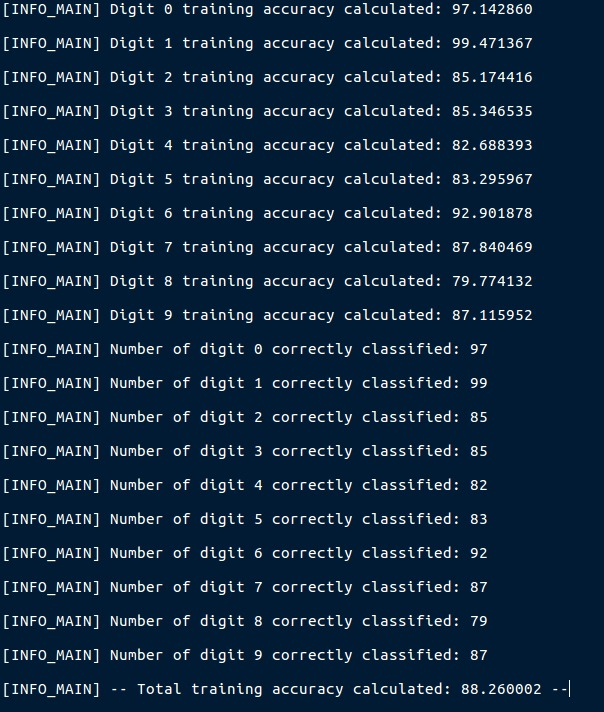
\includegraphics[width=7cm]{OUTPUT1.jpeg}
  \caption{Output para $p=5$ e $m=100$}
\end{figure}

Ou seja, obtemos uma acurácia de aproximadamente 88.2 pct e o programa demorou aproximadamente 27s para executar os treinos e testes.

Rodando para $p=10$ e $m=1000$, obtemos o seguinte output do programa, observado na figura 4.

\begin{figure}[h]
  \centering
  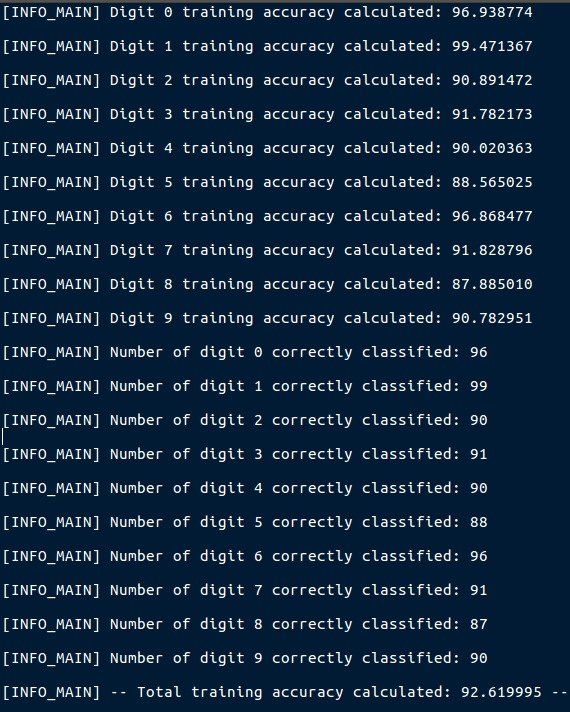
\includegraphics[width=7cm]{OUTPUT2.jpeg}
  \caption{Output para $p=10$ e $m=1000$}
\end{figure}

Nesse caso, observamos uma acurácia de aproximadamente 92.62 pct e o programa demorou aproximadamente 2min13s para executar os treinos e testes.

Por fim, testou-se o programa para o caso de maior número de imagens possíveis de treino. Dessa forma, obtemos o seguinte output, observado na figura 5.

Para essa configuração, o programa consome cerca de 11 minutos para rodar e alcança-se, portanto, uma precisão de aproximadamente 93 pct.

\begin{figure}[h!]
  \centering
  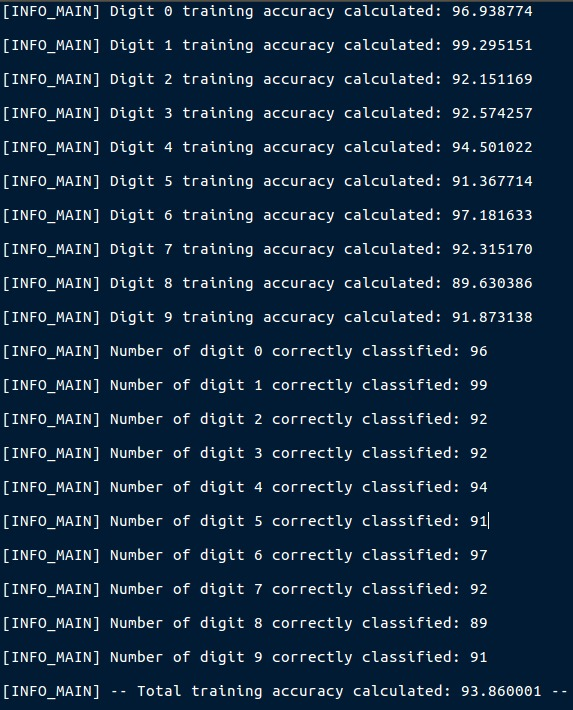
\includegraphics[width=7cm]{OUTPUT3.jpeg}
  \caption{Output para $p=15$ e $m=4000$}
\end{figure}

Notamos que nos três casos, o número 8 apresentou uma precisão menor de classificação. Uma hipótese para isso é o fato do número 8 sofrer uma variação maior na hora da escrita. Dessa forma, é um número que tende a gerar maior divergência de classificação. Por outro lado, o digito 1 foi o que apresentou maior precisão. Por quê? Note que na base MNIST o número "1" é muito padronizado (na maior parte dos casos é uma "barrinha" vertical). Desse modo, por ser bastante padronizado, a acurácia de classificação do digito 1 é bem alta e nos três casos é mais de 99 pct.

Durante os cálculos, o EP1 consome 25 pct de um dos \textit{cores} do processador. Após todos os testes (tarefas e 3 tipos de treino), o EP chegou a consumir cerca de 500mb de memória \textit{RAM}.\\\\\\

\section{Considerações Finais}

Ufa... Depois de três semanas trabalhando nesse projeto, é gratificante os resultados que o mesmo proporciona. Diariamente, trabalhamos com funções de alto nível, como por exemplo Redes Neurais Convolucionais, para resolver problemas de identificação e classificação de imagens. Todavia, muitas vezes, desconhecemos as caixas pretas atrás das bibliotecas. Pensando nisso, a temática do EP1 de Cálculo Numérico nos proporcionou a oportunidade de desvendar mais uma caixa preta do nosso cotidiano e colocar em prática as habilidades computacionais.
Obrigado pela oportunidade! 

\begin{thebibliography}{1}

\bibitem{ref1} SILVA, P. Pedro. {\em Enunciado do EP1 - Machine Learning}. 2019, Instituto de Matemática e Estatística da Universidade de São Paulo.

\bibitem{ref2} SARAIVA, P. Lucas. {\em Notas de aula da disciplina Métodos Numéricos e Aplicações}. 2019, Escola Politécnica da Universidade de São Paulo.

\end{thebibliography}


\end{document}